\section{Procedure And Methods}
\subsection{System Architecture}
\begin{figure*}
	\begin{center}
		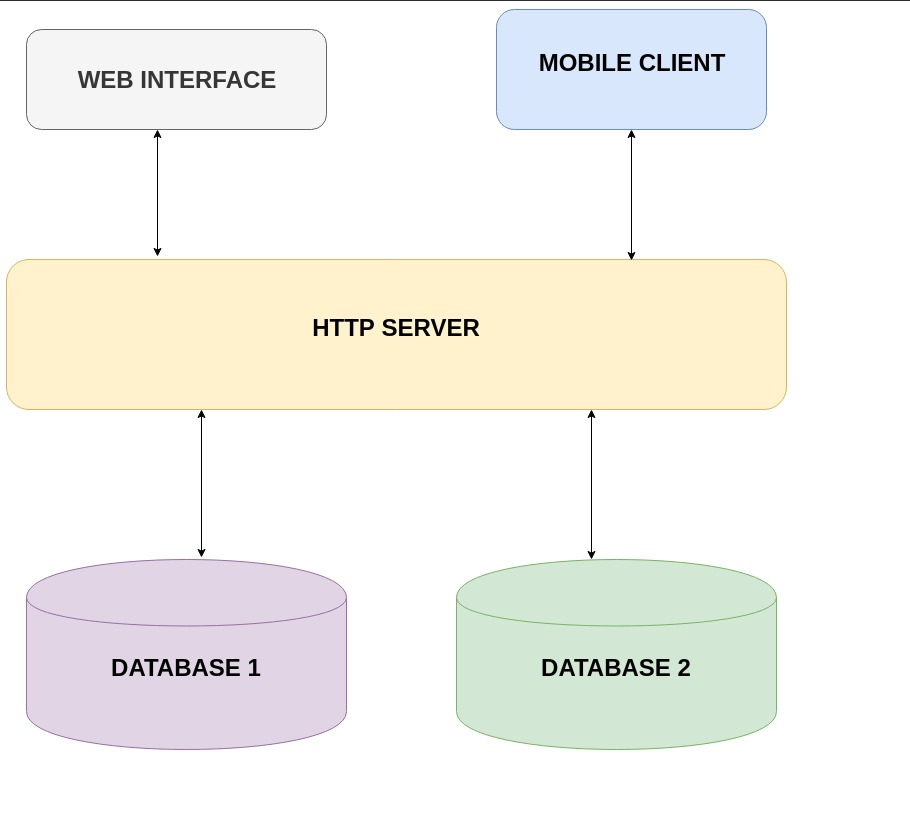
\includegraphics[width=1\linewidth]{res/system.jpeg}
	\end{center}
	\caption{Showing the system overview, different components making the system and the communication directions between these components in the systems.}
	\label{figure:system}
\end{figure*}
Figure ~\ref{figure:system} shows the system over, the components of the system and how everything will fit together. The lines from components are communication lines and suggest the communication direction between the comments. Following is a mapping for each of the line number and the communication information that is sent via that line:
\begin{enumerate}
	\item Request sent from measurement initiator to orchestrator. This is the request for the orchestrator to run measurements on the network. This tool will be useful for researchers who want to carry out measurements on the network for further analysis.
	\item Request sent from data visualizer to the request handler for the data that the visualizer is going to be rendering.
	\item Request from orchestrator to Request handler to so that the request handler can summon the right components for starting network measurement collection process.
	\item In the event that the request handler received a request to run measurement on the network this request has to be sent to a Job scheduler which will add the need to perform measurements on the job queue assuming there are other jobs that will be waiting to be done.
	\item If on the other hand the request is to get data to render on the visualizer, this shows that the request handler needs to send this request to the Database querier to get the data from the database.
	\item This communication link is for queries that are going to be sent t the database system. The information on the queries will specify the database to use and what type of data we are looking for. 
	\item This is the response from the database to be sent to the visualizer.
	\item This line shows the data that comes from a data collector that need to be added to the database through the database query handler. 
	\item From the job scheduler, the job has to be sent to the Job queue so that when ready the job will be sent to the collector via 10 so the collector can initiate the probes to collect measurements.
	\item Shows the job being transfered to the collector from the job queue.
	\item The collector sends the measurement probes alerting them to start collecting measurements.
	\item When the probes are done collecting measurements based on the technique used they will need to somehow send the data to the database. This line will be used to send the data to the collector which will send the data to the database via 8.
	\item Sometimes when the data from the collector has arrived, further measurements may need to be taken for them to make sense,  For this, the network analyzer will have to schedule a new job for collecting measurement.
	\item After the network analyzer get the data it will send the data to the database via this line.
	\item The Database Query handler responds back to the web interface via this line to the response handler.
	\item This line is shows communication from the response handler to the data Visualizer.
\end{enumerate}
The components of the system as seen from the figure ~\ref{figure:system} are:
\paragraph{\textit{Framework Server}}
This is the basis of the application. Other components like the orchestrator and the Collector rely on the server for performing well. The server provides communication to the database system, it also provides a means for scheduling measurements requested via the orchestrator as well as keeping track and ensuring that the jobs are sent to the collector for starting. It also consists of other tools like the request handler which is the communication point from the web interface, the job scheduler that schedules measurement collection jobs for researchers so as not to flood the network with measurement data. it also has a job queue where the scheduled jobs are kept and selected for running at appropriate times. Lastly it provided a component for handling the logic for communicating with the Databases. The reason for having only one central point for database communication is so that if we decided to change the database used, the only aspect form the system that needs to be modified is just this component. We also have a response handler which handles sends responses from the database to the users that they are associated with in the web interface. Lastly, we will have an analyzer of he network data which receives the data from the collector and performs analysis and then saves the data in the database. This part is where the machine learning algorithms can be implemented for making decisions and also adding more jobs on the scheduler.

\paragraph{\textit{Web Interface}}
This consists of the Measurement initiator and the Visualizer tool. From this the users are able to view the network activities in form of graphs. The users are able to also view their profiles which will also be indicated by the visualizer. The measurement initiator is a tool for researchers who want to run network measurements on the network.

\paragraph{\textit{Orchestrator and Collector}}
This are two services that will be running on top of the framework server. These services are responsible for accepting requests from researchers as well as well as initiating measurements form phones and collecting the data from probes.

\paragraph{\textit{Data Collection points}} This consists mobile phones running a Mobiperf extended application. These are where we are measuring the network measurements that will be displayed by the visualizer.
\paragraph{\textit{Database}} Made up of two separate databases for storing measurement data and the other for storing user data.
\subsubsection{Measurement Orchestration}
In terms of orchestration, once measurements are scheduled a job will be stored on the web server with information on the measurement experiment to be run based on user-defined fields such as a number of nodes as well as parameters to measure.When the scheduled time is reached, the Server will send push notifications to online nodes with information on what parameters to be measured. Once the data is collected it will be sent to database 2 ready for viewing through the web interface.
\subsubsection{Network Measurement Collectors}
We need to develop a phone application that will be the means of collecting measurements for the internet metrics. We have decided to build an android application for the phones and tablets as Android is open and requires less resources to get started. According to \cite{statcounter_global_stats}, Android currently has 35\% of the operating systems market. This shows how popular amongst users android is and thus will be a good platform to consider to build the application for first. 
\paragraph{}
The application that we will be building will be extending the MobiPerf application which is built in Java \cite{m-lab}. Since Android Development is also done in Java it also adds to why we will be focusing on developing for android as it is easier to extend an already existing platform compared to creating one form the beginning. The mobile phone are the mobile clients shown on Figure 1. These clients will be talking to the HTTP server to send data to the database or to be triggered to collect network measurements.
\subsubsection{Visualizer}
To design the visualizer, a co-design process will adopted. During the co-design process, about three workshops  will be conducted. A number of users from the Ocean View community will be invited to take part in these workshops. Different Human Computer Interaction methods will be employed to achieve the desired user experience. These will involve both end users and the team taking part in designing and come up with ideas. Co-design is sometimes called participatory design which is defined by \cite{ctx2100202260004041} as a set of theories,practices and studies related to end-users as full participants in activities leading to software products. Thus the reason why we adopted this method as we want to involve users in the design process.
\paragraph{}
The  Django python web framework will be used to build a visualizer web app from the ground up. The framework will be used to implement an HTTP server that will query data from either database1 or database2 as shown on the system design. Data will then be exposed in the form of API endpoints to a front end web framework that will display data in the form of graphs.
\paragraph{}
The advantage of choosing the Django web framework is that it is a simple framework that is easy to use and comes with most back-end functionalities already implemented \cite{10.1007/978-3-540-87403-4_11}. Django also has a lot of support in the Python community, which makes it a reliable option for this project.
\paragraph{}
For the front end, the web app will leverage the react.js a JavaScript front end web framework to build user-friendly interfaces. React is a component-based library which allows rapid prototyping of web applications\cite{Gackenheimer2015}. It also managed by Facebook hence making it a reliable and trustworthy tool to use.
